\section{Summary}

\begin{figure}[H]
\centering
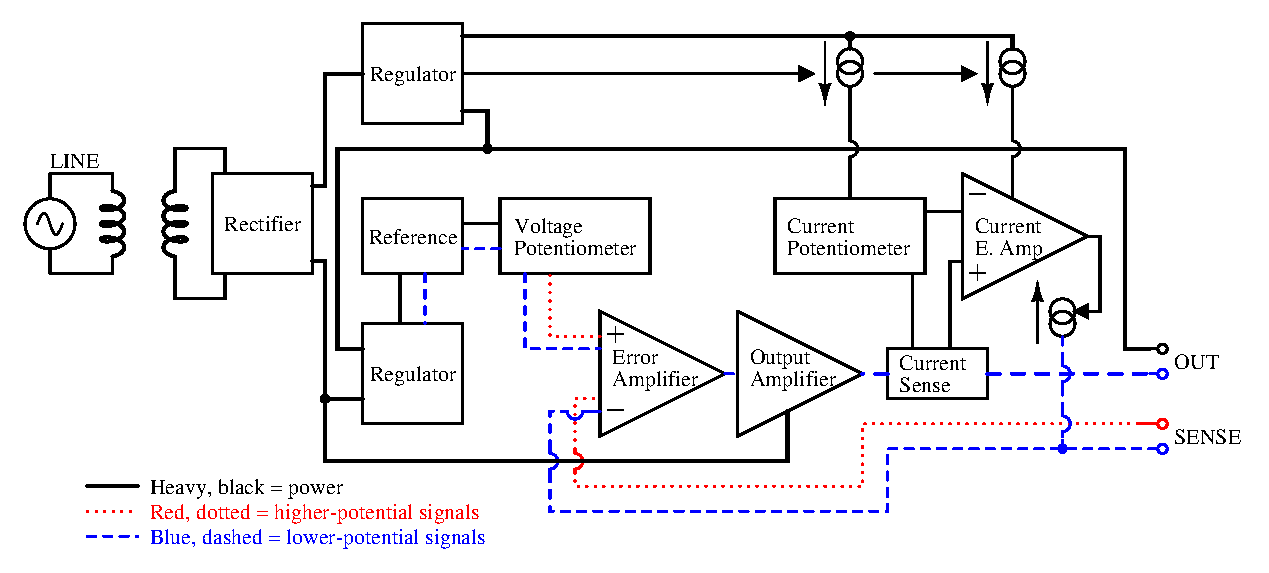
\includegraphics[width=5.5in]{sch/blockdiag}
\caption{Block diagram.}
\label{fig:blockdiag}
\end{figure}

\begin{multicols}{2}

Figure~\ref{fig:blockdiag} is the block diagram of the entire power supply.

First, the line (mains) voltage feeds the primary winding of a transformer,
giving approximately 28~VAC on the secondary.
This is rectified and filtered to DC by diode bridge \texttt{D1} and
capacitor \texttt{C1}.

The current exiting the rectifier passes through a simple ``regulator'',
consisting of just three diodes, to provide a pair of supply rails for
biasing current sources. To maintain good line regulation, the remaining
voltage feeds into a local regulator, giving a rail of approximately -32~V
to power the control circuitry.

This regulated rail powers a Zener reference diode. This regulates the
potential across the front-panel Voltage potentiometer, which is used to select
an output set-point.

The voltage from this potentiometer, as a differential pair, feeds into the
error amplifier, which compares it to the voltage sensed at the output, also as
a differential pair. If the relative voltage between the output pairs is above
that of the set-point, the output drive will be increased; if it is below, the
output drive will be decreased. The output will thus settle to almost exactly
the set-point.

After power leaves the output amplifier, it passes through a current sense
resistor. This resistor sees a potential difference, by Ohm's Law,
corresponding to the current flowing through it. A current sense amplifier
compares this to a current limit set-point; if the current drawn begins to
exceed the set level, the current sense amplifier will pull the negative sense
line further negative.  This causes the voltage amplifier to ``see'' too much
potential on the output, and it decreases output drive.


\end{multicols}
